\chapter{De-Entanglement by additional Divergences - Case study with Emphatic Speech Synthesis}


section{Problem Motivation and Introduction}
Humans exhibit both coarse as well as fine grained explicit control over how they speak an utterance. This targeted control on speech - often manifested in the form of prosodic constructions - allows us to effectively convey our intent in a conversation. Examples of controlled speech generation include simple prosodic manipulations such as implying specific meaning, highlighting or expressing interest in something as well as various communication strategies such as contradiction, contrast, complaints or grudging admiration\citep{nigel_ward_prosodic_patterns}. Further, such manipulation in prosody has been shown effective in
applications such as  Infant Behavior Programs \citep{parental_prosody_changes_mediate_infant_language_production}, improving language acquisition\citep{prosody_functionwords_acquisition} and promoting rapport\citep{rapport_dialogsystems}. It seems natural to employ generative models of speech\citep{tacotron_original,deepvoice2,clarinet,parrotron} to assist in such scenarios \citep{does_tts_help_comprehension}. However, although there has been tremendous progress in the neural generative models for speech in the context of vocoder fidelity\citep{waveglow,wavenet_original}, the notion of controllability in such models is not yet fully evolved. While there have been works towards models aimed at controlling prosody\citep{ tacotron_hierarchical,tacotron_stylefacoruncovering}, the exerted control is still global or coarse grained in terms of styles of speech\citep{tacotron_prosodycontrol,tacotron_styletokens}, etc. In this work, we propose an approach that allows both global as well as local control over the prosodic variation in the generated speech.    

Typically TTS is formulated as a conditional generative modeling problem. In our approach, we propose to instead formulate it as a conditional variational auto-encoder and incorporate automatically derivable information from speech data into the model architecture. This is motivated by the understanding that the utterances themselves do not always contain all the information needed to comprehend the appropriate prosody information. The missing information is either part of background knowledge about the world - implicit to humans but not annotated in the data - or is provided by accompanying context of the utterance. Formulating the task using variational inference allows us to efficiently capture the distribution of prosody thereby avoiding the averaging effect observed in a typical TTS system due to prosody marginalization. To illustrate this, consider an example sentence: `\textit{You do not have a pet shark}'. Most prosodic constructions for this sentence involve sarcasm since it is not commonplace to have sharks as pets - world knowledge. Similarly consider the sentence: `\textit{I dont want to be a nun}'. The linguistic unit subject to realization of prosodic stress in this sentence depends on the context information. Finally, consider the example of a TTS system deployed in a screenreader to assist visually impaired students comprehend math equations. Human voice talent would almost certainly place appropriate prosodic cues that help in comprehension of $x^{(y+z)}$  as opposed to ($x^y + z$). Our formulation allows the model to leverage prosodic information available from the speech signal and capture prosodic distribution. 

To accomplish local as well as global prosody control, we incorporate inductive biases into the model architecture in the form of fundamental frequency($F_0$). Specifically, we quantize $F_0$ into multiple bins and constrain the latent space to disentangle these quantized values from acoustics at the level of phonemes. Our model is explained in detail in section \ref{proposed_approach}. During inference, the prosody distribution can be utilized to control and generate variability in the output speech. In short, our contributions from this work are: (1) We present EDITH, a hierarchical model that disentangles prosodic features in the form of $F_0$ enabling explicit global as well as local control. (2) We show that EDITH captures reliable representation of local prosody by generating speech with desired variations at the chosen linguistic level.  

section{Emphasis by Disentangling Tonal Heuristics(EDITH)}
\label{proposed_approach}

% This is the main section of the paper. This is where the technical novelty of your paper should be clearly explained and motivated. Whenever possible, take the time to remind people how your proposed model/approaches address the challenges highlighted in the introduction. Also, make sure that the novelty of your new approaches is highlighted (i.e., what part was already done vs. what part is novel). You can divide this into two parts - model description and learning. (1) Model Description: formalize mathematically your proposed model or approach. This should include the mathematical definition of the variables involved in your problem (e.g., input variable x and labels y). You should also include an objective function describing what you are modeling (e.g., P(y|x)). While this section may be relatively short (e.g., half a page), you should be consistent with your notation later in the paper. (2) Learning: Describe how you are learning the parameters of your model. State clearly your loss function and the learning algorithm used in your experiments. If you have enough space, give derivation of your gradient, at least for some of the main model parameters.




%In our approach, we propose to incorporate automatically derivable information from speech data into the model architecture so as to enable to Seq2Seq architectures better model prosody. This is motivated by the understanding that the utterances themselves do not always contain all the information needed to comprehend the appropriate prosody information. The missing information is either part of background knowledge about the world - implicit to humans but not annotated in the data - or is provided by accompanying context of the utterance. Consider an example sentence: `\textit{You do not have a pet shark}'. Most prosodic constructions for this sentence involve sarcasm since it is not commonplace to have sharks as pets - world knowledge. Similarly consider the sentence: `\textit{I dont want to be a nun}'. The linguistic unit subject to realization of prosodic stress in this sentence depends on the context information.  While it is possible to include context information in long form content generation such as audiobooks, there are scenarios where we do not have access to the context or the the available context is ambiguous. Consider the example of a TTS system deployed to assist visually impaired students comprehend math equations. There is not sufficient signal in the text to demarcate between  $x^{(y+z)}$ and $x^y + z$. However, human voice talent would almost certainly place appropriate prosodic cues that help in comprehension in such cases. Therefore, we believe that it is helpful to leverage information from the speech signal and incorporate biases into the model architecture during the training itself to help the model accomplish the desired synthesis. 


\begin{figure}[t]
\centering
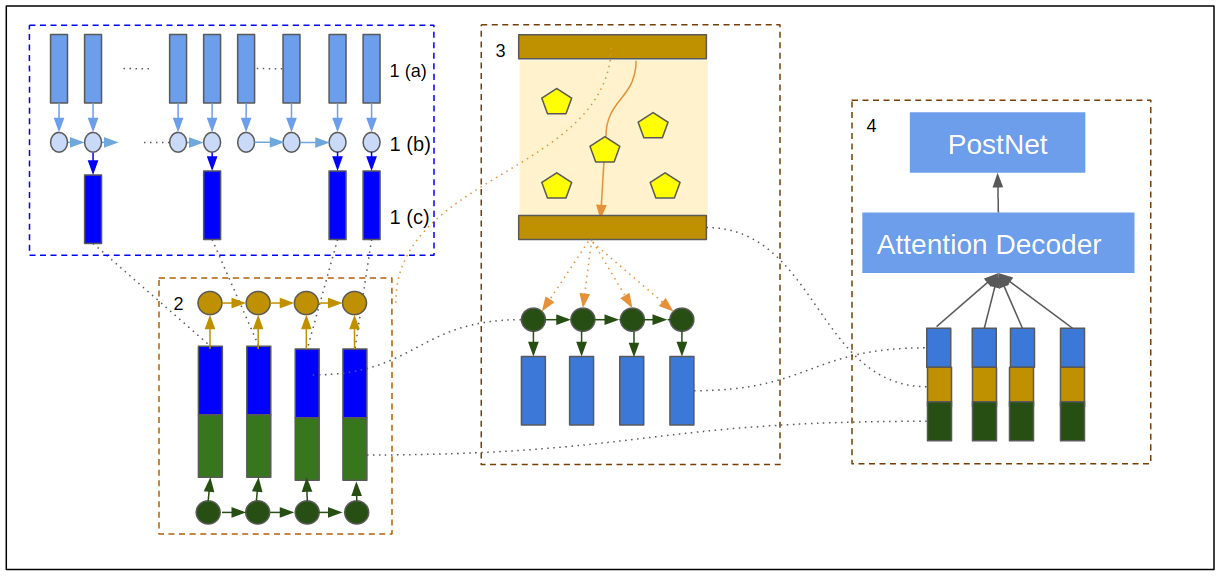
\includegraphics[scale=0.2]{images/EDITH_arch.png}
\caption{\textit{Architecture of EDITH. Circles denote LSTM cells, rectangles represent vectors and pentagons represent global latent vectors. (Best viewed in color)}} 
\label{edith_architecture}
\end{figure}  

EDITH learns the joint distribution between pairs of temporal sequences \{\textbf{x}, \textbf{y}\} where \textbf{x} denotes the features and \textbf{y} denotes the acoustic parameters. Let Ti and To denote the lengths of input and output sequences respectively. Input features \textbf{x} consist of both linguistic features denoted as \textbf{$x_{linguistic}^{1:Ti}$} as well as features extracted from the acoustic signal denoted as \textbf{$x_{acoustic}^{1:To}$}. The output features \textbf{y} consist of linear feature representation \textbf{$y_{linear}^{1:To}$} as well as mel features \textbf{$y_{mel}^{1:To}$}. It has to be noted that \textbf{$x_{acoustic}^{1:To}$} = \textbf{$y_{mel}^{1:To}$}. To efficiently model varying prosody and prevent the averaging effect, we incorporate a variational layer. Therefore, EDITH is a conditional variational auto-encoder. During inference, we discard the encoder part of our model. Our model can be summarized by the following set of equations: 

%section{EDITH: Model Description}


%We are interested in incorporating inductive biases into the architecture of Seq2Seq TTS enabling explicit control over prosody. Ideally, we desire the priors to push model towards learning and exploiting latent representations that can generate different prosodic events. In addition, we also desire the learnt representations to be generalized so that the approach can be extended to different speakers as well as languages or language combinations such as code mixing.  While there are many other parameters associated with prosody, $F_0$ can be considered one of the most important attributes. Based on this, we have chosen to incorporate priors in terms of $F_0$. To accomplish this, we have extracted fundamental frequency using SPTK toolkit\citep{sptk2009speech} and then quantized it into multiple bins with each bin spanning 25 Hz. In other words, continuous $F_0$ values were mapped to their discrete bin indices, resulting in ordinal $F_0$ values for each utterance. We then incorporated these values into the model architecture. We have investigated two ways of incorporating $F_0$ priors: (1) Explicit labeling by directly adding the ordinal $F_0$ as additional input to the model and (2) Implicit incorporation by adding prediction of ordinal $F_0$ as a secondary task in the model. The predicted $F_0$ is used as conditioning information to the decoder along with the input from soft attention. 

%\begin{flalign*}
\begin{equation} \label{eq1}
\begin{split}
encoded ={}& \textbf{H}^{Encoder}(x_{linguistic}, x_{acoustic}) \\
z_{g}, z_{l} ={}& \textbf{VI}(encoded) \\
\hat{y}_{mel} ={}& \textbf{H}^{Decoder}(x_{linguistic},z_{g}, z_{l}) \\
\hat{y}_{linear} ={}& \textbf{H}^{postnet}(\hat{y}_{mel})
\end{split}
\end{equation}
%\end{flalign*}

\iffalse
\begin{equation} \label{eq1}
\centering
\begin{split}
e_{1:T_{input}} & = Encoder(x_{1:T_{input}}) \\
z_{global}, z_{local} = VI(e_{1:T_{input}}) \\
\alpha_{i} & = Attention( e_{1:T_{input}}, d_{i-1}) \\
e^1_i &= \sum_j \alpha_{ij} e_j \\
d_i &= Decoder(e^1_i, s)
\end{split}
\end{equation}
We imagine the generative process as follows:

\begin{itemize}
    \item We sample a global prosody embedding for the utterance.
    \item Conditioned on the sampled embedding and the textual input, we predict local prosody embedding at time $t0$
    \item The predicted prosody embedding is combined with the textual embedding to generate frame level acoustic representation at $t0$.
    \item The process continues.
\end{itemize}

section{Model Components}

\subsubsection{EDITH Encoder}

- clockwork hierarchical LSTM for prosodic features \\
- Vanilla LSTM for linguistic features \\
- Both reset at phone boundaries \\


\subsubsection{EDITH Variational Layer}

- Vector Quantization. \\
- Stop Gradient \\
- Commitment Loss \\
- Normalization of latent vectors

\subsubsection{EDITH Decoder}

- Dot product Attention \\
- 5 frames at once \\
- No masking of outputs to enable better end of sentence prediction.
\fi

Design of our encoder is inpired by the encoder from \citep{chive}. We use clockwork hierarchical LSTM to encode \textbf{$x_{linguistic}^{1:Ti}$} and \textbf{$x_{acoustic}^{1:To}$}. However, our models are clocked at the rate of phones as opposed to syllables. In addition, we do not incorporate any features from word or sentence levels in our encoder to keep the architecture compact. Our variational layer is derived from \citep{vqvae} and is employed  to generate global and local latent variables $z_{g}$, $z_{l}$ respectively. Our decoder is similar to a typical attention based acoustic decoder\citep{tacotron_original} and includes a postnet. While similar in formulation, EDITH has an important difference from \citep{chive} in that our local latent variables follow the rate of input as opposed to output as in \citep{chive}. This allows us to exercise more control over the generated prosodic variations. 

% In \citep{chive}, authors employ clockwork hierarchical decoding for this step. We employ a vanilla architecture instead.

\textbf{Optimization and Learning}: $x_{acoustic}$ is passed through phone rate LSTM. This is shown as block 1 in figure \ref{edith_architecture}. $x_{linguistic}$ is passed through phone LSTM. The representations are concatenated and passed through EDITH Encoder. This is shown as block 2. Outputs from the encoder are passed through the variational layer where vector quantization is performed to pick the most suitable global latent prosodic vector. Conditioned on encoder outputs and the global latent prosodic vector, we predict Ti local prosodic vectors corresponding to predicted local prosodic features. 
We constrain the local latent variables to correspond to quantized $F_0$ by modeling their prediction as a classification task. These local latent variables thus capture the local variations in prosody while global latent variable is reserved for capturing sentence level variations. Ground truth quantized values for classification are obtained by selecting the maximum bin within the duration of phoneme. This is shown as block 3 in the figure. We then employ dot product attention in our decoder. \textbf{$y_{mel}$} is generated by decoder conditioned on local, global latent variables and the encoded $x_{linguistic}$. A postnet is employed to generate \textbf{$y_{linear}$} conditioned on \textbf{$y_{mel}$}. EDITH is optimized to minimize two \textit{L1} losses one each for \textbf{$y_{mel}$} and \textbf{$y_{linear}$} and one classification loss for local latent variables. Additionally, to train the vector quantization layer, we minimize encoder commitment loss for $z_g$ and vector quantization loss following \cite{vqvae} for both $z_g$ and $z_l$. This can be expressed as below:

\begin{equation} \label{eq1}
\begin{split}
\textit{L} = \lambda_{linear} \sum_{t=0}^{To} \| y_{linear}^t - \hat{y}_{linear}^t \|  \\
+ \lambda_{mel} \sum_{t=0}^{To} \| y_{mel}^t - \hat{y}_{mel}^t \| \\
+ \lambda_{qF_0} \sum_{t=0}^{Ti} Div(qF_0, \hat{qF_0}) + \lambda_{e} L_{e} + L_{VQ}\\
\end{split}
\end{equation}


%The weight for the encoder commitment loss is linearly increased to reach 0.2 at update 


\iffalse
\begin{itemize}

    \item $x_{prosodic}$ is passed through phone rate LSTM. This is shown as block 1 in figure \ref{edith_architecture}. Following the approach in \citep{chive}, we reset the state of LSTM after every phoneme boundary.
    \item $x_{linguistic}$ is passed through phone rate LSTM. This is shown as block 2 in figure \ref{edith_architecture}.
    \item The representations are concatenated and passed through EDITH encoder
    \item Outputs from the encoder are passed through the variational layer where vector quantization happens to pick the most suitable global latent prosodic vector. This is shown as block 3 in figure \ref{edith_architecture}.
    \item Conditioned on encoder outputs and the global latent prosodic vector, we predict T local prosodic vectors corresponding to predicted local prosodic features. This is not shown for brevity in the figure.
    \item Global and local latent vectors are then employed in addition to the attention outputs to generate the frame level acoustic features.
    \item Loss Terms : (1) Mel Acoustic feature reconstruction (2) Linear Acoustic feature reconstruction (3) Prosodic Feature Reconstruction (3) Embedding Loss from latent space (4) Encoder commitment loss from latent space 
    
\end{itemize}

\fi


section{Model Interpretation}
This approach can be interpreted as VQVAE\citep{vqvae}. It can also be seen as GST\citep{tacotron_styletokens} based encoding but our approach has two differences:(1) We do not use a different encoder for spectral information and (2) We explicitly constrain the latent classes to correspond to the quantized $F_0$s. We divide the model into individual blocks or modules. Therefore, it can be seen as an extension to Neural Module Networks\cite{neural_module_networks}. In \cite{chive}, authors introduce clockwork hierarchical VAE to predict $F_0$, duration and $C_0$. Our approach of incorporating $F_0$ information at the output of encoder in the form of additional task can be seen similar to this work. However, we use quantized $F_0$s, do not employ clockwork structure in our model and do not explicitly model duration or $C_0$.


section{Experimental Setup}
\label{experimental_setup}

%  Start this section by clearly stating what your main research questions are. Whenever possible, try to design experiments to test specific research hypotheses or questions. If you claimed that components A and B are the main novelties of your model, then you should have ablation experiments that compare your model with and without A (and similarly for B). Your experiments should also include comparison with baseline models (from your midterm report). Furthermore, the experiments should give the reader an understanding of the effect of your model hyper-parameters. For example, plot performance of your model with different regularization factors. Finally, make sure to write the experimental setup method in such a way that a person not familiar with your work would be able to reproduce your model just by reading the paper. Describe the dataset you are using for this project. Describe the input modalities and annotations available in this dataset. Describe your experimental methodology for evaluating the baseline model(s). This should include the way you split your dataset for training, validation and testing. It should also include any details about the hyper-parameters and the evaluation metrics. If space is too short, you can move some of the implementation details in the supplementary material, but the main design decision should be explained in the main paper.



\textbf{Data}: We have used data from LJSpeech dataset\citep{ljspeech_dataset} to build our systems. We have used all of the 13100 sentences. The text was normalized manually to convert non standard forms (for ex. 1993) to written forms (nineteen ninety three).


\iffalse
section{Baseline}

Our acoustic model is based on Tacotron\cite{tacotron_original} Seq2Seq speech synthesis system and is built using PyTorch. We have used phones as the input instead of characters.  We have not performed masking of padded frames as is typically done in Seq2Seq models. We found that not masking helps model better predict end of sentence as mentioned in \cite{tacotron_original}. Since adjacent frames seem to be correlated, our decoder predicts 3 frames per timestep. We have used a batch size of 64 to train the baseline model. 
\fi
%Our vocoder is based on WaveNet\cite{wavenet_original}. Speech signal was power normalized and squashed to the range (-1,1). We have used 16 bit mulaw quantization to encode individual samples. Instead of transposed convolutions we have employed linear interpolation to upsample the acoustic frames to match the time resolution of speech samples. To optimize the model, we use discretized Mixture of Logistics loss\cite{salimans2017pixelcnn++,juvela2019waveform} with 12 logistic classes. 


\textbf{Baselines}: Our acoustic model is based on Tacotron\cite{tacotron_original} Seq2Seq speech synthesis system is built using PyTorch\citep{pytorch}. We have not performed masking of padded frames as is typically done in Seq2Seq models. We found that not masking helps model better predict end of sentence as mentioned in \cite{tacotron_original}. Since adjacent frames seem to be correlated, our decoder predicts 5 frames per timestep. Our model has three deviations from the original implementation: (1) Phones are used as the input instead of characters. (2) CBHG module in the encoder and postnet has been replaced with with three LSTM layers. (3) We use all the predicted frames at a time step as input to the decoder(as opposed to only the last time step) while predicting the next frames.  We have used a batch size of 64 to train the baseline model. To enable control of prosody, we employ quantized $F_0$ values as additional inputs to this baseline model. For this, we first extract $F_0$ values for the dataset and quantize them into multiple bins each spanning 25 \textit{Hz} without any overlap. These quantized $F_0$ values are embedded and added as additional inputs to the baseline model. In other words, this is a conditional generative model with phones and quantized $F_0$s as inputs. Additionally, we also build a model that uses word level prosodic features extracted using AuToBI\citep{rosenberg2010autobi}. We refer to this system as \textbf{AuToBI}.

\textbf{EDITH Hyperparameters}: The encoders of both $x_{acoustic}$ and $x_{linguistic}$ are realized using bidirectional LSTMs. We have used 256 as the hidden dimensions for both these encoders. Both our global and local latent variables are of 256 dimensions. We employ 10 global latent classes. The network to predict local latent variables is implemented using bidirectional LSTMs that takes 512 dimensional input and outputs 256 dimensional vectors. Encoder weight $\lambda_e$ was linearly increased to 0.2 till 10K timesteps and remained constant after that. For quantization of $F_0$, we have followed the same procedure as in Baseline. 25 Hz was chosen as the size of bin. This effectively resulted in a total of 14 bins and thus 14 local latent classes. After every update step, we normalize the local latent variables by the norm. Since these classes correspond to ordinal data in terms of quantized $F_0$s, we believe that normalizing places the vectors on a unit circle.

\textbf{SubUtterance Models}: Long utterances present in audiobooks  are rich in prosodic variations but also lead to computational overhead in terms of processing speed. Therefore, we have built systems that have access to only part of the utterance by selecting aligned segments of text and acoustics within a full sentence. We note that such an approach is already used for vocoding: Typical vocoders the authors are aware of are trained using aligned chunks of acoustic vectors and corresponding speech samples  as opposed to full utterances. Encouraged by this, we build sub utterance based models for both baseline as well as proposed approach. To distinguish from the full sentence models, we refer to these systems as Sub Utterance Baseline(\textit{SUB}) and Sub Utterance EDITH(\textit{SUE}) while referring to the full sentence models as Full Utterance Baseline(\textit{FUB}) and Full Utterance EDITH(\textit{FUE}) respectively.

%We have built multiple variants to compare the performance of the proposed approach. Extending our baseline, we have built systems that employ quantized F0 in their architectures. Additionally, we have also built models trained with access to only part of the full sentence. We refer to these systems as Full Sentence Quantized F0 (FSQ) and Sub Sentence Quantized F0 (SSQ) respectively. For each of the above systems, we have incorporated the prior information about F0 either at the input or as an additional loss term after the encoder. We refer to these systems with subscripts. For instance, the system employing full sentences for training with quantized F0 as inputs in addition to phoneme embeddings is referred to as $FSQ_i$. Similarly, the system employing sub sentence training but with additional loss term is referred to as $SSQ_l$. In addition to the proposed approaches, we have also built systems that employ AuToBI\cite{rosenberg2010autobi} labels. We have not built a sub sentence variant in this approach and refer to the full sentence variant as AUTOBI. We have utilized 1300 sentences as validation data to tune our hyperparameters.

\begin{table}[t]
\centering
\caption{\textit{Results from Preference and MOS Tests for Emphasis generation. The entries for the preference portion(columns 2 through 6)indicate preference values obtained by the systems in the first column against every other system in the subsequent columns.}} 
\small
\setlength\tabcolsep{2pt}
\begin{tabular}{|c|c|c|c|c|c|| c| }
  \hline
 Config &  $FUB$ &  $FUE$ & $SUB$ & $SUE$ & AUToBI & MOS\\
  \hline
  $FUB$ &  -  & 92 & 396 & 363 & \textbf{441} & 4.0\\
  \hline
  $FUE$(ours) &  \textbf{345} & - & \textbf{424}  & \textbf{378} & \textbf{477} & 4.0 \\
  \hline
 $SUB$ &  91 & 86 & - & 235 & \textbf{278} & 3.4 \\
  \hline
 $SUE$(ours) &  64 & 86 &  243 & - & 227 & 3.6 \\
  \hline
 AUToBI &  47 & 19 & 219 & 256 & - & 3.9 \\
  \hline
\end{tabular}
\label{table_results_quantvsautobi}
\end{table}

\textbf{Evaluation}:
Evaluation was performed  in the form of listening tests using \citep{testvox_parlikar}. We have conducted two types of listening tests: (1) Rating the naturalness in  terms of Mean Opinion Score (MOS) on a scale of 1(least natural) to 5(highly natural) and (2) ABX Preference test on Emphasis where the users need to mention their preference towards either of the systems or state that they prefer neither. For the preference evaluation we have manually curated 50 sentences where the meaning was implied based on prosody. Participants were shown the entire sentence and its implication in parenthesis. An example sentence from our testset is `\textit{It looks like a starfish} (but it really is not).' Every system was used to generate this test set\footnote{in the mentioned example, the systems generated just the part '\textit{It looks like a starfish}' and not the part in parenthesis}. For baseline and proposed approaches, the phonemes to be emphasized are rendered with embedding vector corresponding to bin 12 while others are rendered with bin 8 The participants are to mention their preference to the system that faithfully generates prosody in line with the information in parenthesis. We had 25 listeners and each participant rated 20 random sentences giving us a total of 500 ratings per pair of systems.


\begin{figure}[t]
\centering
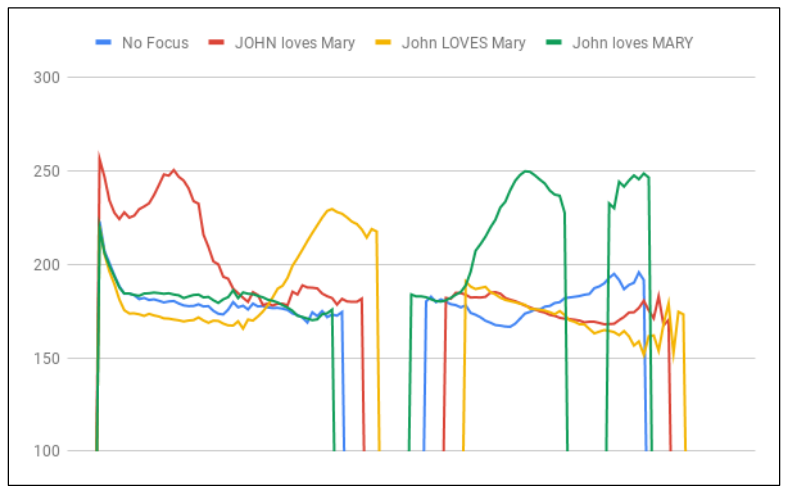
\includegraphics[scale=0.25]{images/f0_manipulation.png}
\caption{\textit{Plot of Fundamental Frequency($F_0$) trajectories obtained from generated waves using proposed approach \textit{FUE}. Variants of the sentence `John loves Mary' are generated with emphasis on individual words(captialized). The blue trajectory corresponds to $F_0$ when no emphasis was applied to any word. The plot highlights that the proposed approach allows explicit local control at the desired level in the generated speech. We have submitted the generated wavefiles as supplementary material.}} 
\label{plot_overview}
% These and other samples are attached in the supplementary material for reference.
\end{figure}  



\textbf{Discussion}: The preference evaluation results for the proposed approaches are presented in table \ref{table_results_quantvsautobi}.  We have excluded the \textit{No Preference} values from this table for brevity. However, they can be estimated based on the values in the table. The full utterance based systems seem to outperform sub utternace as well as AuToBI based systems consistently. Within the full sentence systems,  our proposed approach(\textit{FUE}) outperforms the baseline conditional generative model(\textit{FUB}). A sample output generated by conditioning the local latent variables to emphasize individual linguistic units(words) from our approach can be examined in figure \ref{plot_overview}. An informal listening test in the scenarios where full sentence models were not preferred revealed an interesting finding: All these scenarios were when the emphasized word was the first in the sentence. We hypothesize that this might be due to the canonical word order(\textbf{SVO}) in English. One approach to handle this could be to incorporate a suitable weighting to consider this effect and we plan to investigate this further.  The sub utterance based approaches seem to match the performance of AUToBI systems while clearly under performing their full utterance counterparts. Informal listening evaluations revealed that the sub utterance models seem to have repetition of phoneme units within the generated sentence. We attribute this to the errors in alignment and phoneme boundary estimation and plan to investigate approaches to circumvent this behavior in future work. 

%Some listeners have expressed that they felt multiple words were focused in the sentence but nevertheless the intended word more or less stood out from the rest except when it was the first word in sentence. We hypothesize that this might be due to the data distribution and plan to investigate this further. 

section{Conclusion}

In this case study, we have proposed an approach to obtain local and fine grained control over prosody in neural generative models for speech. For this we quantize fundamental frequency, which is highly correlated with prosody information, into multiple bins. We infer this information employing hierarchical global and local latent variables in the model architecture.  We show that our approach generates appropriate emphasis at word level and significantly outperforms AuToBI in terms of flexibility.  
